\documentclass[10pt]{article}

% Preamble

\usepackage{amsmath,amsfonts,amssymb}
\usepackage[mathscr]{euscript}
%\usepackage[mathcal]{euscript}
\usepackage{mathrsfs}
\usepackage{graphicx}
\usepackage{float}
\usepackage{bbm}
\usepackage{braket}
\usepackage{tikz-feynman}
\usepackage{simpler-wick}
\usepackage{cancel}
\usepackage{stackengine}
\usepackage{slashed}
\usepackage{caption}
\usepackage{pgfplots}

\newcommand{\bigzero}{\mbox{\normalfont\Large\bfseries 0}}

\title{Notes On Introduction to Conformal Field Theory \\ A Course Given By Dr. Tobias Osborne}
\author{Transcribed by Dr. Alexander V. St. John}

% The Document

\begin{document}

\maketitle

\clearpage

\section*{Lecture 1: Introduction to Conformal Field Theory}
\label{sec: lec1}

\noindent Recommended references:

\begin{itemize}
\item \textit{A Mathematical Introduction to Conformal Field Theory} by Schottenloher.
\item \textit{Applied Conformal Field Theory}, hep-th/9108028, by Ginsparg.
\item \textit{Conformal Field Theory} (``Yellow Book'') by Francesco, Mathieu, Senechal.
\end{itemize}

\noindent Why study conformal field theory (CFT)?

\begin{itemize}
\item CFT provides a good description of systems at or near criticality.
\item CFTs are the only true quantum field theories (QFTs), since they are cutoff-independent. One can think of QFTs as perturbations of CFTs. CFTs correspond to renormalization groups of fixed points, which dominate an effective theory at or near criticality.
\item CFTs can be made, by and large, mathematically rigorous, at least in $(1+1)$-dimensional theories. There are three major competing mathematical descriptions for CFT, and advances are being made towards a single, unifying description.
\end{itemize}

\noindent Prerequisites for this material:

\begin{itemize}
\item Advanced quantum mechanics
	\subitem E.g, many-body theory and Fock spaces.
\item Classical field theory
	\subitem E.g., symplectic geometry.
\item Quantum field theory.
\item Advanced quantum field theory.
\end{itemize}

\noindent What is CFT?

\begin{itemize}
\item A \textit{conformal field theory} is a field theory, quantum or classical, that is invariant, or symmetric, under a group of transformations called the \textit{conformal group} $G$.
\item In a classical field theory, this means that the equations of motion are left invariant.
\item In a quantum field theory, this means that, by Wigner's theorem, there is a projective unitary representation of the group $G$. In other words, symmetries, or transformations, that leave the transition amplitude invariant, are realized, up to a phase, by (anti)unitary operators.
\end{itemize}

\subsection*{Conformal Transformations in $d$ Dimensions}

\noindent Let $M = \mathbb{R}^{p,q}$ be a manifold $\mathbb{R}^d$, where $d = p+q$, and $p,q \in \mathbb{Z}_{\ge 0}$. To this manifold, assign the metric

\begin{equation}
g_{\mu\nu} \equiv \eta_{\mu\nu} = \text{diag} (1,1,\dots,1,-1,-1,\dots,-1)
\end{equation}

\noindent With the first $p$ entries equal to one, and the last $q$ entries equal to minus one. Note that this is not necessarily a Riemannian metric, since the signature can be negative. We have a few cases of interest for this metric

\begin{itemize}
\item $p=d$ , Riemannian.
\item $p = d-1$, $q=1$, Lorentz.
\item $q > 1$, e.g., $q=2$, AdS-CFT correspondence.
\end{itemize}

\noindent A conformal transformation leaves the metric invariant up to a scale factor. \\

\noindent Consider a smooth change of coordinates

\begin{equation}
x \rightarrow x' = x' (x) \text{ , with } x = (x^1, x^2, \dots, x^p, x^{p+1}, \dots, x^{p+q})
\end{equation}

\noindent Such that the metric, a type-$(2,0)$ tensor, undergoes an \textit{active coordinate} transformation as

\begin{equation}
g_{\mu\nu} (x) \rightarrow g'_{\mu\nu} (x') \equiv \frac{\partial x^\alpha}{\partial x'^\mu} \frac{\partial x^\beta}{\partial x'^\nu} g_{\alpha \beta} (x') 
\end{equation}

\noindent And then impose the condition

\begin{equation}
g'_{\mu\nu} (x') = \Omega (x') g_{\mu\nu} (x').
\end{equation}

\noindent Where $\Omega(x) > 0$ is the (local) scale factor. Note that if the scale factor is zero, then we have a singularity, which we will discuss later. A transformation that obeys the last line is called \textit{conformal}, and these transformations preserve angles

\begin{equation}
\angle \theta = \frac{g_{\mu\nu} u^\mu v^\nu}{\sqrt{(g_{\mu\nu} u^\mu v^\nu)^2}}.
\end{equation}

\noindent The \textit{conformal group} of a manifold M is denoted by $\text{Conf}(M)$, and is the connected component of the group of all conformal transformations of $M$ containing the identity, in a compact, open topology. \\

\noindent So, in a quantum conformal field theory, we are looking for a Hilbert space $\mathcal{H}$ and a projective unitary representation of the group $G$ for \textit{local} QFTs

\begin{equation}
G \rightarrow \pi (G).
\end{equation}

\noindent This is unexpectedly nontrivial, and makes for a very rich field of study, since there is a tension between knowing the unitary representations of symmetries and demanding that the representation is locally implementable. \\

\noindent To classify the conformal group on our chosen manifold $G = \text{Conf} (\mathbb{R}^{p,q})$, consider an infinitesimal conformal (active coordinate) transformation on the spacetime coordinates

\begin{equation}
x^\mu \rightarrow x'^\mu = x^\mu +  \epsilon^\mu (x)
\end{equation}

\noindent Which must leave the metric invariant up to the scale factor $\Omega(x)$. This places constraints on $\epsilon$ (\textbf{Exercise}) \\

\begin{equation}
g_{\mu\nu} \rightarrow g'_{\mu\nu} = g_{\mu\nu} + (\partial_\mu \epsilon_\nu + \partial_\nu \epsilon_\mu) + \mathcal{O} (\epsilon^2).
\end{equation}

\noindent To satisfy the constraint placed by conformal invariance on the metric (c.f., $g_{\mu\nu} \rightarrow g'_{\mu\nu} (x') = \Omega(x') g_{\mu\nu} (x')$), as well as the constraint that the conformally transformed metric is still proptional to the diagonal flat spacetime metric $g'_{\mu\nu} \propto \eta_{\mu\nu}$, we must have that the second term is also diagonal, proportional to $\eta_{\mu\nu}$

\begin{align}
(\partial_\mu \epsilon_\nu + \partial_\nu \epsilon_\mu) &\propto \eta_{\mu\nu} \\
\implies (\partial_\mu \epsilon_\nu + \partial_\nu \epsilon_\mu) &= \text{constant} \cdot \eta_{\mu\nu}
\end{align}

\noindent Take the trace of each side, set $\mu=\nu$, and solve for the constant

\begin{equation}
\text{constant} = \frac{2 (\partial \cdot \epsilon)}{d}
\end{equation}

\noindent So, the conformal transformation on the metric reads, tossing out higher order terms,

\begin{equation}
g'_{\mu\nu} = g_{\mu\nu} + \frac{2 (\partial \cdot \epsilon)}{d} g_{\mu\nu}.
\end{equation}

\noindent And substituting into the proportionality relation from above, we have

\begin{equation}
(\partial_\mu \epsilon_\nu + \partial_\nu \epsilon_\mu) = \frac{2}{d} (\partial \cdot \epsilon) \eta_{\mu\nu}.
\end{equation}

\noindent Combining this with the conformal transformation of the metric and comparing to the metric transformation law, we get that the scale factor $\Omega(x)$ for the conformal transformation of the spacetime metric is 

\begin{equation}
\Omega(x) = 1+\frac{2}{d} (\partial \cdot \epsilon).
\end{equation}

\noindent Then it follows from $(\partial_\mu \epsilon_\nu + \partial_\nu \epsilon_\mu) = \frac{2}{d} (\partial \cdot \epsilon) \eta_{\mu\nu}$ , expanding and equating mixed partial derivatives to third order, and we get $d^2$ partial differential equations of the form (\textbf{Exercise})

\begin{equation}
(\eta_{\mu\nu} \Box + (d-2) \partial_\mu \partial_\nu) (\partial \cdot \epsilon) = 0
\end{equation}

\noindent Where $\Box = \eta^{\mu\nu} \partial_\mu \partial_\nu$ is the d'Alembertian operator.

\subsubsection*{Classification of Infinitesimal Conformal Translations for $d>2$}

\noindent By examining the condition for $\epsilon$ and the $d^2$ equations

\begin{align}
(\partial_\mu \epsilon_\nu + \partial_\nu \epsilon_\mu) &= \frac{2}{d} (\partial \cdot \epsilon) \eta_{\mu\nu} \\
(\eta_{\mu\nu} \Box + (d-2) \partial_\mu \partial_\nu) (\partial \cdot \epsilon) &= 0
\end{align}

\noindent We find that third order derivatives of $\epsilon(x)$ vanish and $\epsilon(x)$ is at most quadratic. \\

\noindent This leaves four types of infinitesimal transformations, defined via $\epsilon$, allowable in a conformal transformation: one constant, two linear, and one quadratic in spacetime coordinates.

\begin{enumerate}
\item Spacetime translations
	\subitem $\epsilon = a^\mu$.
\item Rotations
	\subitem  $\epsilon^\mu = \omega^\mu_{\,\,\nu} x^\nu$, $\omega$ antisymmetric.
\item Scale transformations
	\subitem $\epsilon^\mu = \lambda x^\mu$, $\lambda > 0$.
\item Special conformal transformations (SCT; inversion through a sphere)
	\subitem $\epsilon^\mu = b^\mu x^2 - 2 x^\mu (b \cdot x)$.
\end{enumerate}

\noindent Note that Lorentz and Poincar\'e transformations are always subgroups of the conformal group, leaving the metric invariant. since $\omega$ corresponds to boosts and Euclidean affine rotations complete the Poincar\'e group. \\

\noindent \textbf{Theorem} \\

\noindent Every conformal transformation that acts on an connected subset of Minkowski space, including the whole space itself, $\varphi : \, U \subset \mathbb{R}^{p,q}$, where $p+q > 2$, is a composition of 

\begin{itemize}
\item a translation
	\subitem $x^\mu \rightarrow x^\mu + a^\mu$, where $a \in \mathbb{R}^d$,
\item an orthogonal transformation (rotation)
	\subitem $x \rightarrow \Lambda x$, where $\Lambda \in O(p,q)$,
\item a dilation (scale)
	\subitem $x^\mu \rightarrow \lambda x^\mu$, where $\lambda \in \mathbb{R}^+$,
\item and an SCT
	\subitem $x \rightarrow \frac{x^\mu - b^\mu x^2 }{1-2b \cdot x + b^2 x^2}$, where $b \in \mathbb{R}^q$.
\end{itemize}

\noindent Note that it is possible to find a vector $b$ such that the denominator is equal to zero, the SCT is not invertible, and this is no longer a group. Also note that if we don't compactify the space and include $\infty$ as a point available to the conformal transformation, the group becomes significantly smaller and more constrained. \\

\subsubsection*{Classification of Infinitesimal Conformal Translations for $d=2$}

\noindent If $d=2$, the spacetime metric becomes the identity

\begin{equation}
g_{\mu\nu} = \delta_{\mu\nu}
\end{equation}

\noindent And $(\partial_\mu \epsilon_\nu + \partial_\nu \epsilon_\mu) = \frac{2}{d} (\partial \cdot \epsilon) \eta_{\mu\nu}$ becomes the Cauchy-Riemann equations and $\epsilon(x)$ is complex-valued, complex-differentiable, and analytic

\begin{equation}
\partial_1 \epsilon_1 = \partial_2 \epsilon_2 \text{ and } \partial_1 \epsilon_2 = - \partial_2 \epsilon_1.
\end{equation}

\noindent Introduce the complex coordinates

\begin{equation}
z = x^1 + i x^2 \text{ and } \bar{z} = x^1 - i x^2.
\end{equation}

\noindent Then we can complexify $\epsilon$ as

\begin{equation}
\epsilon(z) = \epsilon^1 + i \epsilon^2 \text{ and } \bar{\epsilon}({\bar{z}}) = \epsilon^1 - i \epsilon^2.
\end{equation}

\noindent Two-dimensional global, gotten via exponentiation of an infinitesimal transformation, conformal transformations correspond to \textit{entire} (no singularities, invertible everywhere), \textit{holomorphic} functions $z \rightarrow f(z)$ with holomorphic inverses $f^{-1} (z)$. The only allowable form for a conformal transformation that corresponds to an entire, holomorphic function is linear in the complex coordinates

\begin{equation}
f(z) = \alpha z + \beta, \text{ where } \alpha, \beta \in \mathbb{C}.
\end{equation}

\noindent We may expect a larger group of symmetries with entirety and holomorphism enforced, since the space seems less constrained, but this actually constrains the space more and the group becomes smaller. So, if we were to not compactify, and add infinity as a point, as we demonstrated, the conformal space becomes linear and boring: only rotations and scaling are allowed.\\

\noindent To include this complex representation of the spacetime coordinates, we \textit{extend} our manifold to the complex numbers $\mathbb{C}$ and compactify complex space to a Riemann sphere $\mathbb{C} \cup \{ \infty \}$ we get the proper space for the conformal transformations to act in

\begin{equation}
\mathbb{R}^{2,0} \rightarrow \mathbb{C} \rightarrow \mathbb{C} \cup \{\infty\} \rightarrow \text{Conf}(\mathbb{C} \cup \{\infty\} )
\end{equation}

\begin{figure}[H]
	\centering
	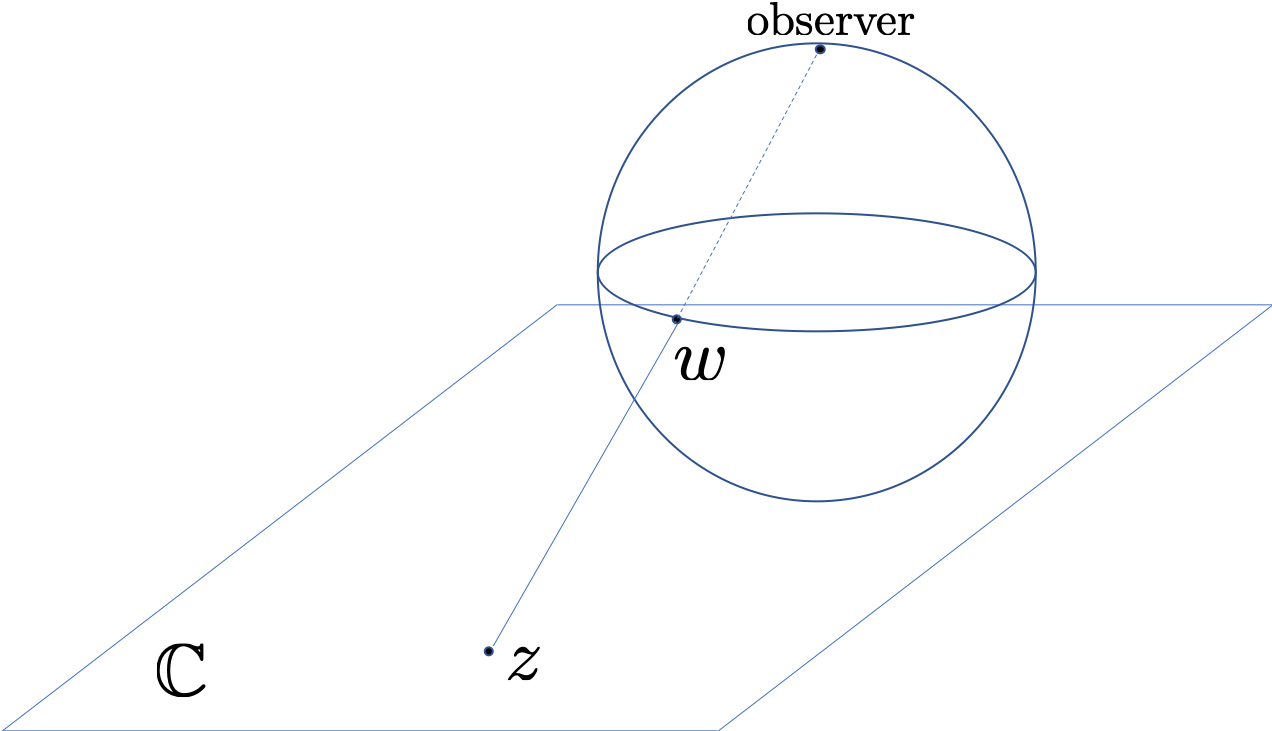
\includegraphics[width=3in]{images/riemann_sphere.png} 
\end{figure} 

\noindent Where the conformal group is

\begin{equation}
\text{Conf}(\mathbb{C} \cup \{ \infty \} ) = \Big{\{} f(z) = \frac{\alpha z + \beta}{\gamma z + \delta}; \, \alpha, \beta, \gamma, \delta \in \mathbb{C}, \alpha\delta - \beta \gamma \ne 0 \Big{\}}.
\end{equation}

\noindent This is also called the group of Moebius transformations, and is a slightly larger group of conformal transformations (symmetires), since we can map to and from infinity as a point. \\

\subsubsection*{Summary}

\noindent A conformal field theory is a local quantum field theory that is invariant under the conformal group, a set of transformations, a change in coordinates, that leave the metric invariant up to a scale factor. In different spacetime dimensions, the conformal group takes on significantly different forms. \\

\noindent The global conformal group in dimensions greater than two is comprised of translations, rotations, scaling, and special conformal transformations, as well as dimensions equal to two, as long as the space is compactified. If singularities are included, functions with poles are allowed, the symmetry gets larger.


\clearpage

%\section*{Lecture 2: }
%\label{sec: lec2}

%
\noindent In the last lecture we introduced global conformal transformations/symmetries of some manifold $M$ that form a (symmetry) group $G$ which can be promoted to a symmetry group of some quanutm system, where the kinematics of the system are described by a Hilbert space $\mathcal{H}$. The quantum system is said to be globally conformally invariant if these is some unitary representation, operators $U$ that act on the Hilbert space,

\begin{equation}
U: \,\, G \rightarrow U(\mathcal{H}).
\end{equation}

\noindent Recall that in the generalized Minkowski space $\mathbb{R}^{p,q}$, the structure of the group of global conformal transformations $G$ consists of compositions of translations, dilations, rotations(boosts), and special conformal transformations (SCTs). \\

\noindent Here we now study the case where $d=2$, which will expand our notion of what a symmetry is and will allow us to define local, infinitesimal conformal transformations. \\

\noindent For example, a global conformal transformation, a $1-1$ differentiable map from $\mathbb{R}^2 \rightarrow \mathbb{R}^2$, may consist of a dilation and a rotation and look like

\begin{figure}[H]
	\centering
	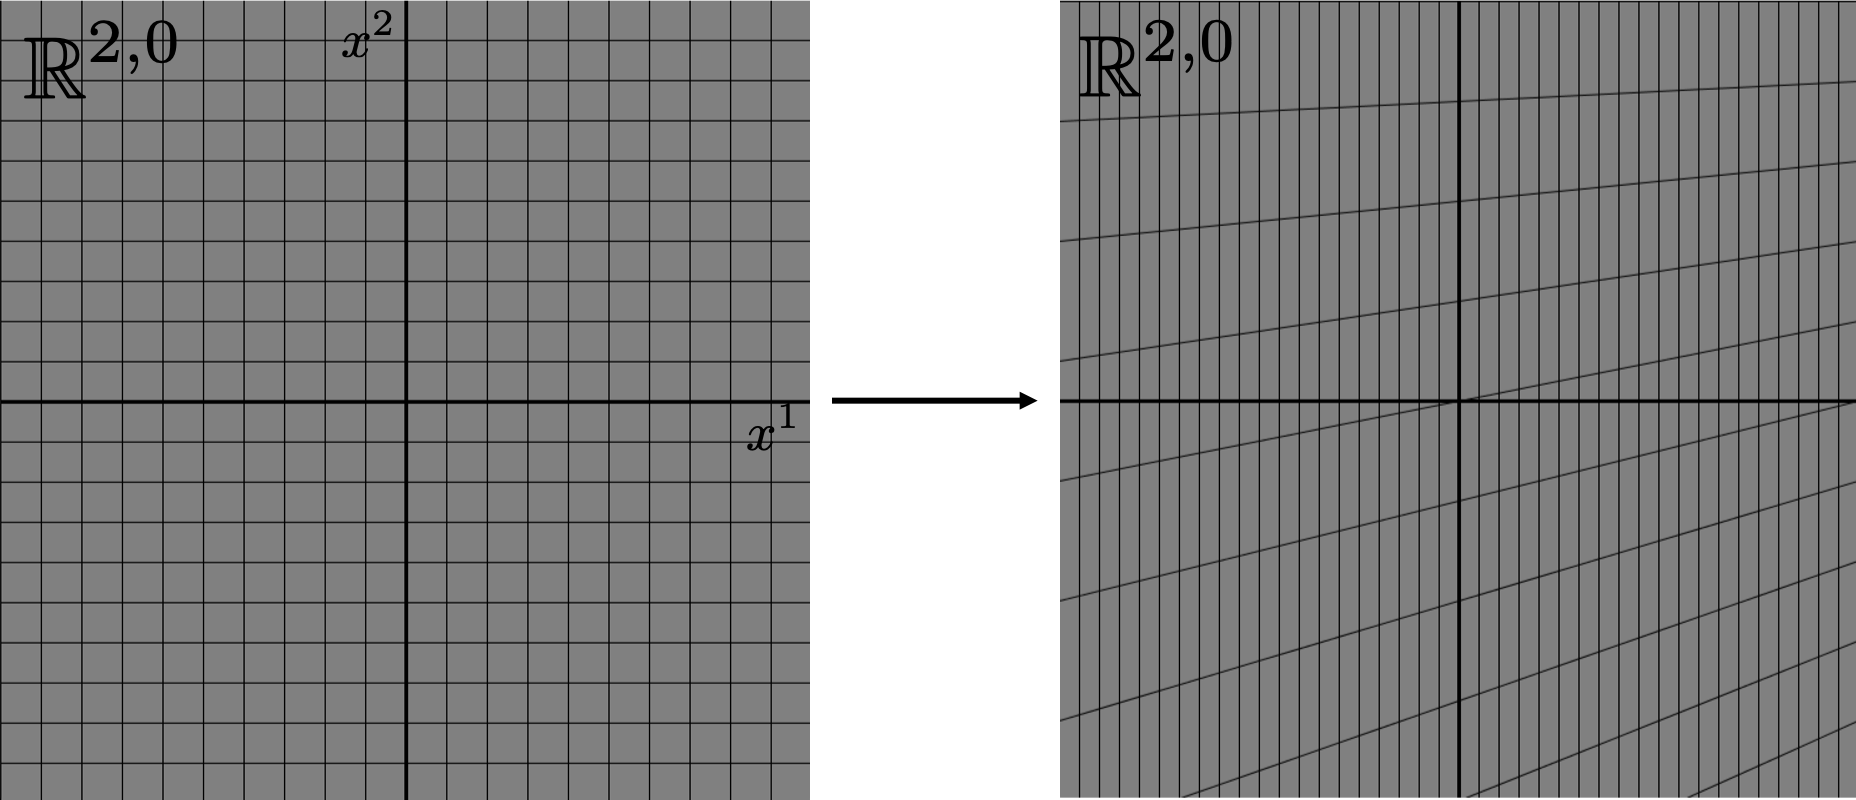
\includegraphics[width=4in]{images/global_conf_trans.png} 
\end{figure} 

\noindent For contrast, consider an infinitesimal conformal transformation $\text{id} + \epsilon X$, where $X=X(x)$ is a vector field, the derivative of a diffeomorphism, that acts on the two-dimensional Minkowski space as

\begin{figure}[H]
	\centering
	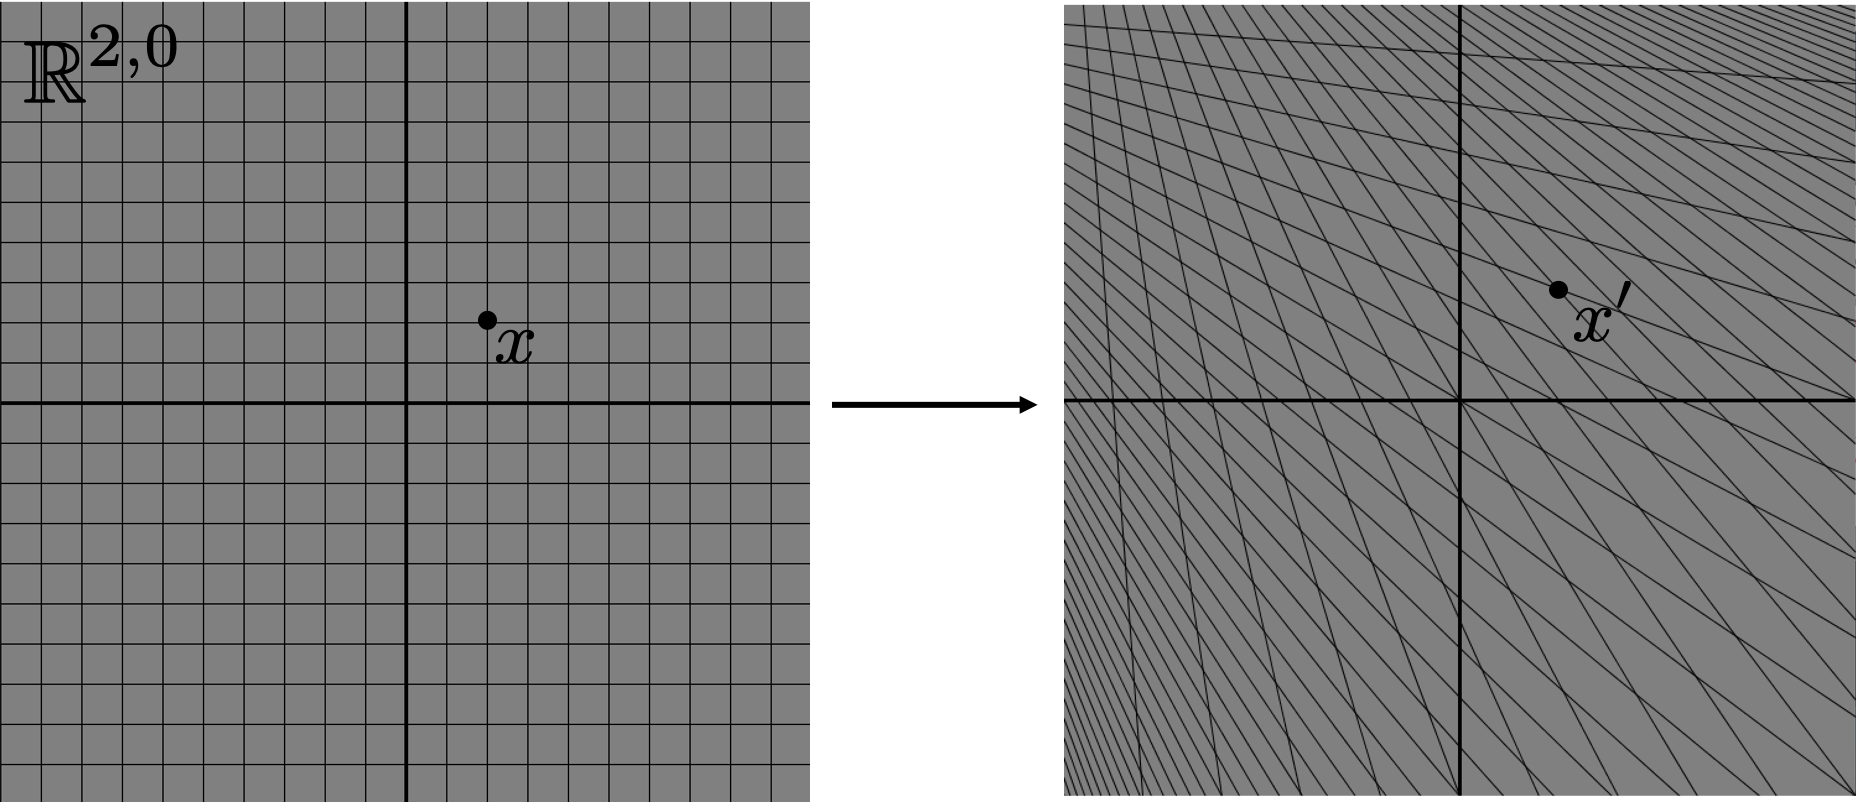
\includegraphics[width=4in]{images/inf_conf_trans.png} 
\end{figure} 

\noindent This transformation preserves all of the right angles in the untransformed Minkowski space, and the action is close to the identity, such that $|x-x'| \sim \mathcal{O}(\epsilon)$. The transformation $\text{id} + \epsilon X$ is conformal to first order in $\epsilon$, as is required by the definition of infinitesimal. \\

\noindent Although the vector field $X(x)$ is a generator of the infinitesimal conformal transformation, it does not necessarily define a global transformation via exponentiation, as it just may not be well defined globally.\\

\noindent To begin to make sense of this, consider in quantum mechanics, where we talk about quantum systems symmetric under a group $G$ with HIlbert space 

\begin{equation}
(\mathcal{H}, \,\, U: \, G \rightarrow U(\mathcal{H})).
\end{equation}

\noindent So, in quantum mechanics, we are reduced to finding these unitary representations of $G$. If $G$ is finite, it does not make sense to speak infinitesimally (e.g., one one-hundredth of a reflection). \\

\noindent We assume $G$ is a manifold, and then we may as well go as far to assume that $G$ is a Lie group with an associated Lie algebra $\mathfrak{g}$, which consists of vector fields that exponentiate to the Lie group. Then the quantum system is symmetric under the Lie algebra if you get a representation

\begin{equation}
(\mathcal{H}, \, \, \pi: \, \mathfrak{g} \rightarrow L(\mathcal{H}))
\end{equation}

\noindent Where $L(\mathcal{H})$ is the set of (bounded and unbounded) linear operators, and $\pi$ generates a unitary operator on the Hilbert space, such that $\pi(X)= e^{isX}$, $s\in \mathbb{R}$. \\

\noindent Note that for an infinite-dimensional group, (1) the operator $e^{isX}$ may not be continuous, and (2) the Lie algebra may not exponeniate to a Lie group, which we will encounter in conformal field theory. In other words, in contrast to when we used infinitesimal quanities to build global representations, we find that infinitesimal conformal transformations don't necessarily exponentiate to a group.\\

\noindent Therefore, in the infinitesimal case, we abandon looking for (full, continuous) unitary representations of the Lie group, and instead focus in on finding Hermitian representations that generate the Lie algebra. \\

\subsection*{Local algebra of infinitesimal conformal transformations}

\noindent Recall that for global conformal transformations, we have $z \rightarrow f(z)$, where $f$ is holomorphic with inverse $f^{-1}$. For infinitesimal $f$, this transformation, including the complex conjugate, becomes

\begin{equation}
z \rightarrow z + \epsilon (z) \text{ and } \bar{z} \rightarrow \bar{z} + \bar{\epsilon}(\bar{z})
\end{equation}

\noindent Where $\epsilon$ is a holomorphic function. A convenient choice of basis, which is infinite dimensional, is

\begin{equation}
\epsilon_n (z) = -\epsilon z^{n+1} \text{, where } n \in \mathbb{Z}.
\end{equation}

\noindent Given a diffeomorphism $[z \rightarrow z + \epsilon_n (z)] = e^{\epsilon \ell_n}$, the corresponding vector field tangent to every point in the manifold is defined by the operators

\begin{equation}
\ell_n \equiv - z^{n+1} \partial_z \text{ and } \bar{\ell}_n \equiv - \bar{z}^{n+1} \partial_{\bar{z}}.
\end{equation}

\noindent These differential operators form a basis, since they obey the commutation relations (\textbf{Exercise})

\begin{align}
[ \ell_m , \ell_n ] &= (m-n) \ell_{m+n} \\
[ \bar{\ell}_m, \bar{\ell}_n ] &= (m-n) \bar{\ell}_{m+n} \\
[\bar{\ell}_m , \ell_n ] &= 0.
\end{align}

\noindent They also as form a closed, infinite-dimensional Lie algebra $\forall m,n \in \mathbb{Z}$, called the Witt algebra $\text{WItt} = \mathcal{A} \oplus \bar{\mathcal{A}}$, where $\mathcal{A}$ is generated by $\{ \ell \}$, and $\bar{\mathcal{A}}$ is generated by $\{ \bar{\ell} \}$. Everything commutes in the basis, so the direct sum of the Witt algebra is justified. \\

\noindent The Witt algebra is generated infinitesimally, and could also be used to infinitiseimally generate a Lie group. This turns out to be true, but the Lie group is not the conformal group. \\

\noindent Which operators $\ell_n$ correspond to global transformations? \\

\noindent Consider a vector field 

\begin{equation}
v(z) = - \sum_{n=-\infty}^{\infty} v_n \ell_n = \sum_{n=-\infty}^{\infty} v_n z^{n+1} \partial_z.
\end{equation}

\noindent For this vector field to correspond to a global transformation, $v(z)$ must exponentiate to a holomorhpic map $f$, which is nonsingular in the limit as $z \rightarrow 0$. This places constraints on the coefficients of the vector field 

\begin{equation}
v_n = 0, \, n < -1.
\end{equation}

\noindent The inverse of the vector field must also exponentiate to a holomorphic map $f^{-1}$, which is nonsingular in the limit as $z \rightarrow \infty$ (e.g., exists on the Riemann sphere). This places the constraint on the coefficients of the vector field: 

\begin{equation}
v_n = 0, \, n>1.
\end{equation}

\noindent Note that if we demand holomorphism on the full complex plane without compactifying, the only allowed global transformations will be linear transformation (\textbf{Exercise}). By compactifying $\pm \infty$ as a point onto the Riemann sphere, we have more freedom in allowed global transformations. \\

\noindent With these constraints in place, we are left with three (six with complex conjugates) generators of infinitesimal global conformal transformations

\begin{equation}
\ell_{-1}, \ell_0 , \ell_1 \text{ and } \bar{\ell}_{-1}, \bar{\ell}_0, \bar{\ell}_1.
\end{equation}

\noindent The generators close to form a subalgebra under the commutator bracket $[,]$ defined above (\textbf{Exercise}), and generate thegroup of \textit{linear fractional (Moebius) transformations}, also known as the projective special linear group $\text{PSL}(2,\mathbb{C})$

\begin{equation}
z \rightarrow \frac{az + b}{c z + d}, \,\, ad-bc = 1.
\end{equation}

\noindent The set of global conformal transformations allowed in this basis are (\textbf{Exercise}), for $s \in \mathbb{R}$,

\begin{align}
&\text{Translation: } &e^{s \ell_{-1}} \equiv &\begin{pmatrix}1&-s \\ 0&1 \end{pmatrix} &\equiv z \rightarrow z - s \\
&\text{Dilation: } &e^{s (\ell_0 + \bar{\ell}_0)} \equiv &\begin{pmatrix}\lambda&0 \\ 0&\lambda^{-1} \end{pmatrix} &\equiv z \rightarrow e^{-s} \\
&\text{Rotation: } &e^{is (\bar{\ell}_0 - \ell_0)} \equiv &\begin{pmatrix}\text{exp}(i\frac{\theta}{2})&0 \\ 0&\text{exp}(-i\frac{\theta}{2}) \end{pmatrix} &\equiv z \rightarrow e^{is} \\
&\text{Special: } &e^{s \ell_1} \equiv &\begin{pmatrix}1&0 \\ c&1 \end{pmatrix} &\equiv z \rightarrow \frac{z}{1+sz}.
\end{align}

\noindent Note that for $\mathbb{R}^{d,0}$, $d>2$, the local transformations are also global! Also note that in one-dimensional spacetime, $(1,0)$ or $(0,1)$, conformal transformations are all monotonic increasing functions $\mathbb{R} \rightarrow \mathbb{R}$.

\subsection*{$d=2$ Minkowski space, $\mathbb{R}^{1,1}$}

\noindent The conformal group  of $\mathbb{R}^{1,1}$ is \textit{special}. \\

\noindent \textbf{Theorem:} \\

\noindent A smooth map $\varphi = (u,v) : \, M \rightarrow \mathbb{R}^{1,1}$ from a connected subset of $M \subset \mathbb{R}^{1,1}$ is conformal (pulls back metric to a scalar multiple of the diagonal metric), iff $u_x^2 > v_x^2$ and $u_x = v_y,\, u_y = v_x$ or $u_x = -v_y,\, u_y = -v_x$. \\

\begin{figure}[H]
	\centering
	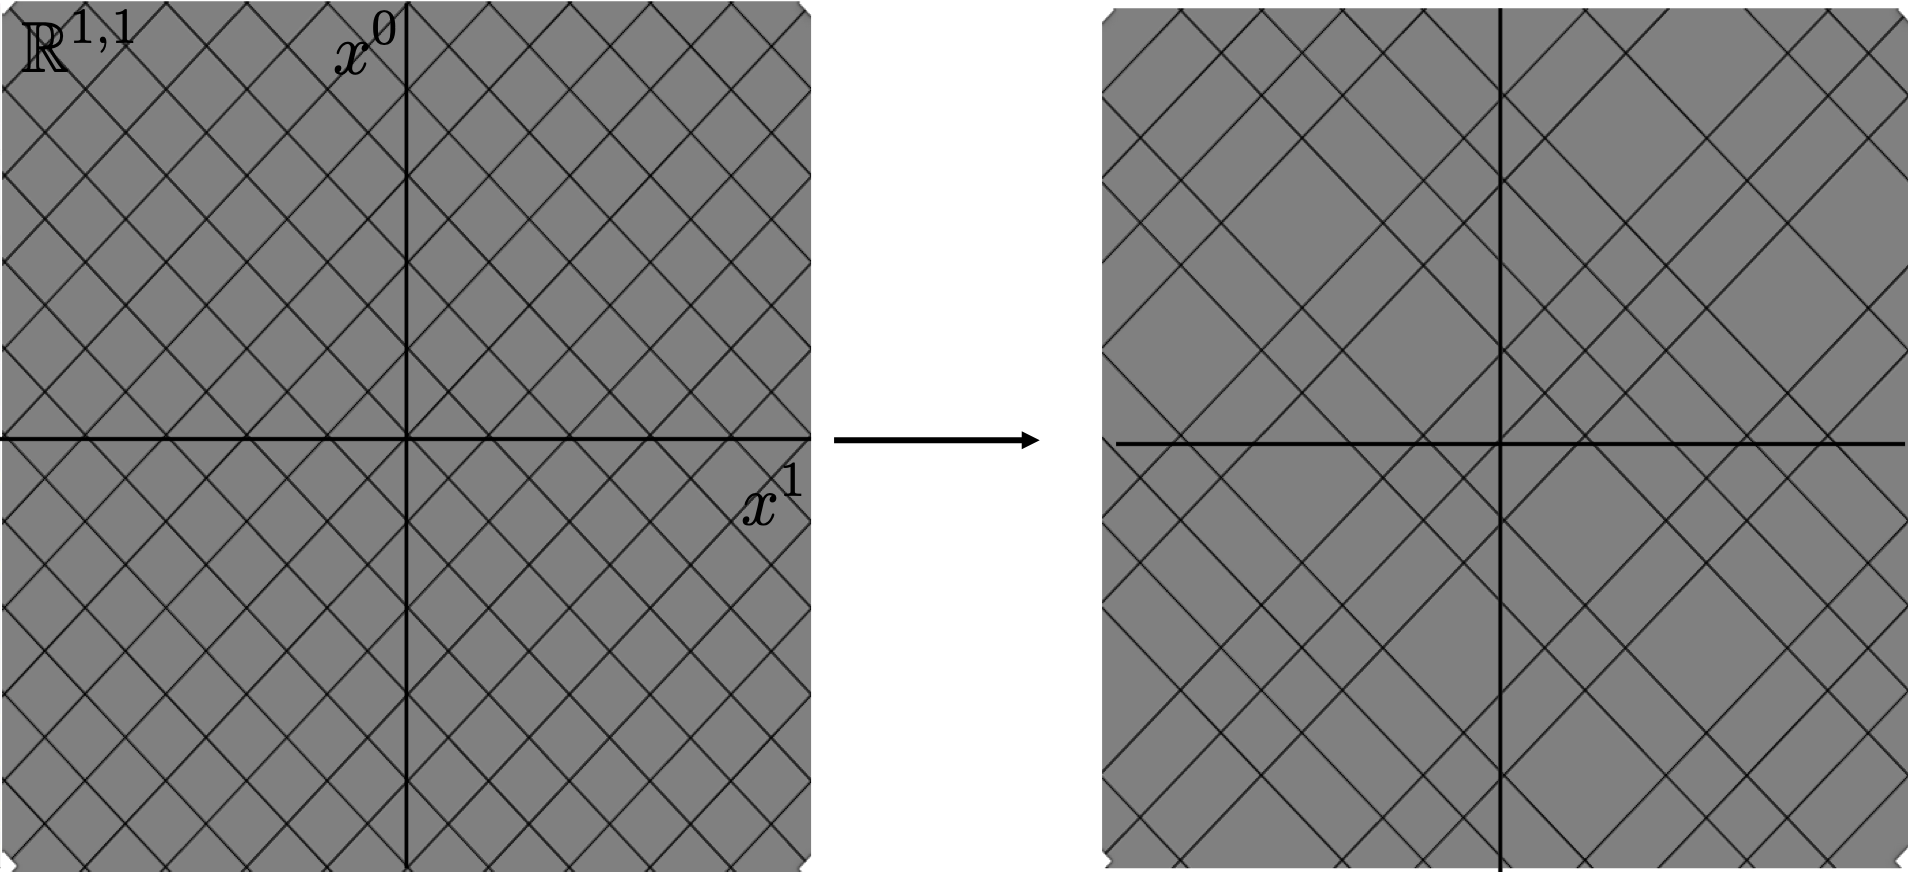
\includegraphics[width=4in]{images/conf_trans_lightcone.png} 
\end{figure} 

\noindent \textbf{Theorem:} \\

\noindent Consider an infinitely differentiable function on the real line $f \in C^\infty (\mathbb{R})$, and let $f_\pm \in C^\infty (\mathbb{R}^2, \mathbb{R})$, the infinitely differentiable functions from the real line to the real plane, be defined by $f_\pm (x,y) = f(x \pm y)$. Then the map 

\begin{align}
\Phi: \, C^\infty (\mathbb{R}) \times C^\infty (\mathbb{R}) &\rightarrow C^\infty (\mathbb{R}^2, \mathbb{R}^2) \\
(f,g) &\rightarrow \frac{1}{2} (f_+ + g_-, f_+ - g_- )
\end{align}

\noindent Has the following properties

\begin{itemize}
\item image($\Phi$) $= \{ (u,v): \, u_x = v_y, \, u_y, v_x \}$
\item $\Phi(f,g)$ is conformal iff $f'>0$ and $g' >0$ or $f'<0$ and $g'<0$
\item $\Phi$ is bijective iff $f$ and $g$ are bijective
\item $\Phi(f \circ h, g \circ k) = \Phi(f,g) \circ \Phi (h,k), \forall f,g,h,k \in C^\infty(\mathbb{R}) \equiv \Phi$ is a homomorphism.
\end{itemize}

\noindent The group of orientation-preserving transformations of $M=\mathbb{R}^{1,1}$ is isomorphic to 

\begin{equation}
(\text{Diff}_+ (\mathbb{R}) \times \text{Diff}_+ (\mathbb{R})) \cup (\text{Diff}_- (\mathbb{R}) \times \text{Diff}_- (\mathbb{R}))
\end{equation}

\noindent Which consists of the infinitely-differentiable orientation-preserving maps of $\mathbb{R}$, diffeomorphisms of $\mathbb{R}$. \\

\noindent It is convenient to compactify $\mathbb{R}^{1,1} \rightarrow S^{1,1} \subset \mathbb{R}^{2,0} \times \mathbb{R}^{0,2}$. Then the group of orientation-preserving transformations of $M=S^{1,1}$ is isomorphic to 

\begin{equation}
\text{Conf} (\mathbb{R}^{1,1}) \equiv (\text{Diff}_+ (S^1) \times \text{Diff}_+ (S^1)) \cup (\text{Diff}_- (S^1) \times \text{Diff}_- (S^1)).
\end{equation}

\noindent This is the definition of the conformal group of Minkowski space. Typically, we throw away the second part of the union, the $''-''$ reversing part, since it is the same as preserving with $z \rightarrow -z$, and focus on the infinite-dimensional subgroup $\text{Diff}_+ (S^1)$, which we call the \textit{chiral half} of the conformal group. This is admissable, since the symmetries of a quantum system can be understood by the symmetries of $\text{Diff}_+ (S^1)$, and the rest is easily gotten by tensor products to include the other light-cone axes. \\

\noindent In the next lecture, we will focus on which quantum systems are invariant under this infinite-dimensional group $\text{Diff}_+ (S^1)$ by going to the Lie algebra, which turns out to be isomorphic to the Witt algebra, in the Euclidean case. The unitary representations, gotten via infinitesimal generators, of $\text{Diff}_+ (S^1)$ will not be bounded below and are unstable. Therefore, \textit{projective} unitary representaitons will be required, and are classified by the \textit{central charge}.

%\clearpage



\end{document}